\chapter{Результаты}\label{res}

\section{Поиск следов отбора в гене \textit{CYTB}}

На первом этапе мы использовали 62 последовательности гена \textit{CYTB} представителей всех основных родов и триб Arvicolinae. Среди них были почти все филогенетически неродственные виды, перешедшие к существованию в подземной среде: представители рода \textit{Ellobius}, \textit{P. schaposchnikowi}, \textit{L. mandarinus}, \textit{T. subterraneus} и \textit{M. pinetorum}. Сравнение проводилось с наземными видами из 22 родов (рис. \ref{PhyloTree} и приложение А). 

\subsection{Поиск параллельных аминокислотных замен}

При анализе изменчивости гена\textit{CYTB} мы нашли три паралельные замены, характерные для подземных грызунов: Ser57Pro, Asp214Asn и Ile338Val (рис. \ref{PhyloTree}). Замена Asp214Asn была обнаружена также и у специализированных подземных грызунов из других семейств.

\begin{figure}[h!]
	\begin{center}
		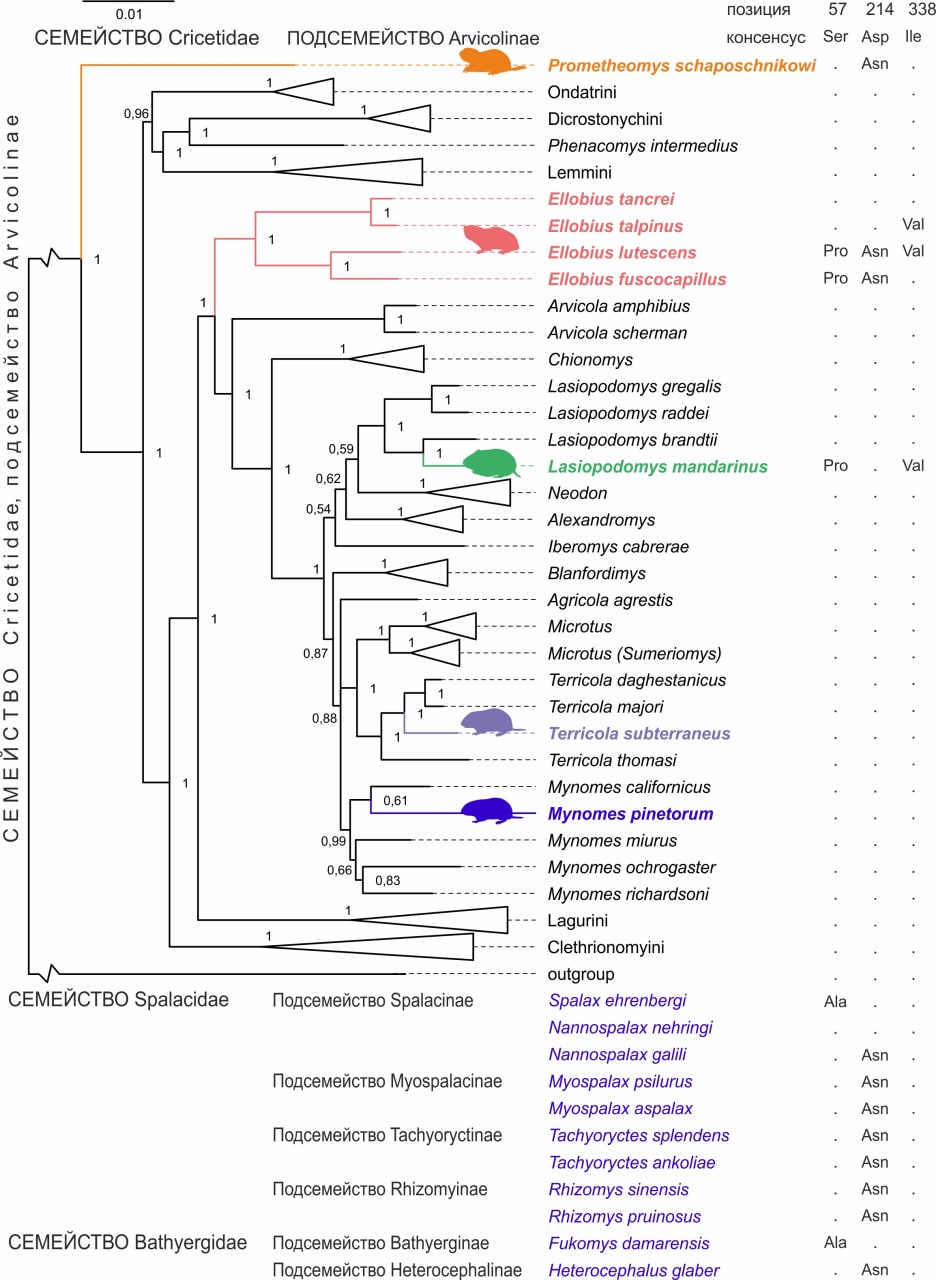
\includegraphics[width=0.9\textwidth]{Cytb_tree_colour_ed}
	\end{center}
	\caption{Филогенетическое дерево взятых в анализ видов. Указаны аминокислотные замены, характерные для подземных видов. Подземные виды отмечены цветом.}
	\label{PhyloTree}
\end{figure}

\clearpage

Замена серина на пролин в остатке 57 у подземных грызунов потенциально удаляет сайт фосфорилирования. Мы использовали два разных метода, чтобы оценить статус фосфорилирования этого сайта. Сервер NetPhos 3.1 предсказал фосфорилирование киназой \textit{CDC2} с оценкой 0,518. GPS 5.0 выявил киназы \textit{AGC}, \textit{PKN} и \textit{PKN1} с оценкой 65,363. Предсказания киназ не согласуются друг с другом, однако все прогнозы указывают на высокую вероятность фосфорилирования этого сайта. Те же методы не предсказывали фосфорилирование для Asp214Asn, и, насколько нам известно, ни Ile, ни Val в позиции 338 не могут быть фосфорилированы.

Нуклеотидная замена в кодоне 338 (ATT> GTT), приводящая к замене Ile338Val, была обнаружена как вероятный патоген в базе данных ClinVar и связана с раковыми процессами: www.ncbi.nlm.nih.gov/clinvar/variation/143898/.

Мы смоделировали третичную структуру белка цитохрома, чтобы изучить возможный структурный эффект замен (рис. \ref{CytStructure} A). Согласно ей, Ser57 обращен к межмембранному пространству митохондрий. Он расположен на неструктурированном сегменте петли, охватывающем остатки 54–60. Эта петля контактирует с той же петлей на втором мономере цитохрома \textit{bc1} в комплексе (рис. \ref{CytStructure} B). В отличие от Ser57Pro, замещение Asp214Asn находится на петле, обращенной к матрице митохондрии. Он контактирует с N-концом субъединицы VII комплекса убихинол-цитохром с редуктазы III (UQCRQ) (рис. \ref{CytStructure} C). Замена Ile338Val находится на границе раздела $\alpha$-спиралей в трансмембранной области комплекса (рис. \ref{CytStructure} D). Смоделированная структура показывает, что эта замена благоприятствует другому ротамеру Ile350, который соседствует с остатком 58 UQCRQ.

\begin{figure}[h!]
	\begin{center}
		\includegraphics[width=0.8\textwidth]{fig структура}
	\end{center}
	\caption{Структурная модель замен в комплексе цитохрома \textit{bc1}. \textbf{A.} Обзор гомодимера цитохрома \textit{bc1}. Цитохром Б --- голубой, UQCRQ - пурпурный. Второй мономер окрашен в желтый цвет. Места замены выделены кружками. IMS --- межмембранное пространство. \textbf{B.} Увеличенные структуры \textit{E. lutescens} и \textit{L. sibiricus}, показывающие замену Ser57Pro. Модель \textit{E. lutescens} голубая, \textit{L. sibiricus} --- белая. \textbf{C.} Замена Asp214Asn и его взаимодействие с N-концом UQCRQ (пурпурный) \textbf{D.} Замена Ile338Val и соседняя цепочка UQCRQ (пурпурный)}
	\label{CytStructure}
\end{figure}

Для рассмотрения внутривидового аминокислотного полиморфизма в сайтах, выявленных программой TreeSAAP, был взят расширенный набор данных: 6 059 последовательностей \textit{CYTB} для наземных видов и 131 -- для подземных. Он включал в себя все, что было в базе данных GenBank по взятым в анализ видам на август 2020 года. Сравнение частот использования аминокислот в каждой позиции белка выявило более 60 сайтов, в которых есть достоверные различия между подземными и наземными видами (таблица \ref{BigTable}). Среди них были обнаруженные в ходе анализа TreeSAAP позиции 57 и 338.

%рисунок с распределением замен

\subsection{Оценка уровня отбора}
Оценка значений $\omega$ (отношение \textit{dN/dS}) у взятых в анализ видов показала общую тенденцию к ослаблению уровня отбора у подземных грызунов при сравнении их с филогенетически близкими наземными видами (рис. \ref{Tree4Selection})


\begin{figure}[h!]
	\begin{center}
		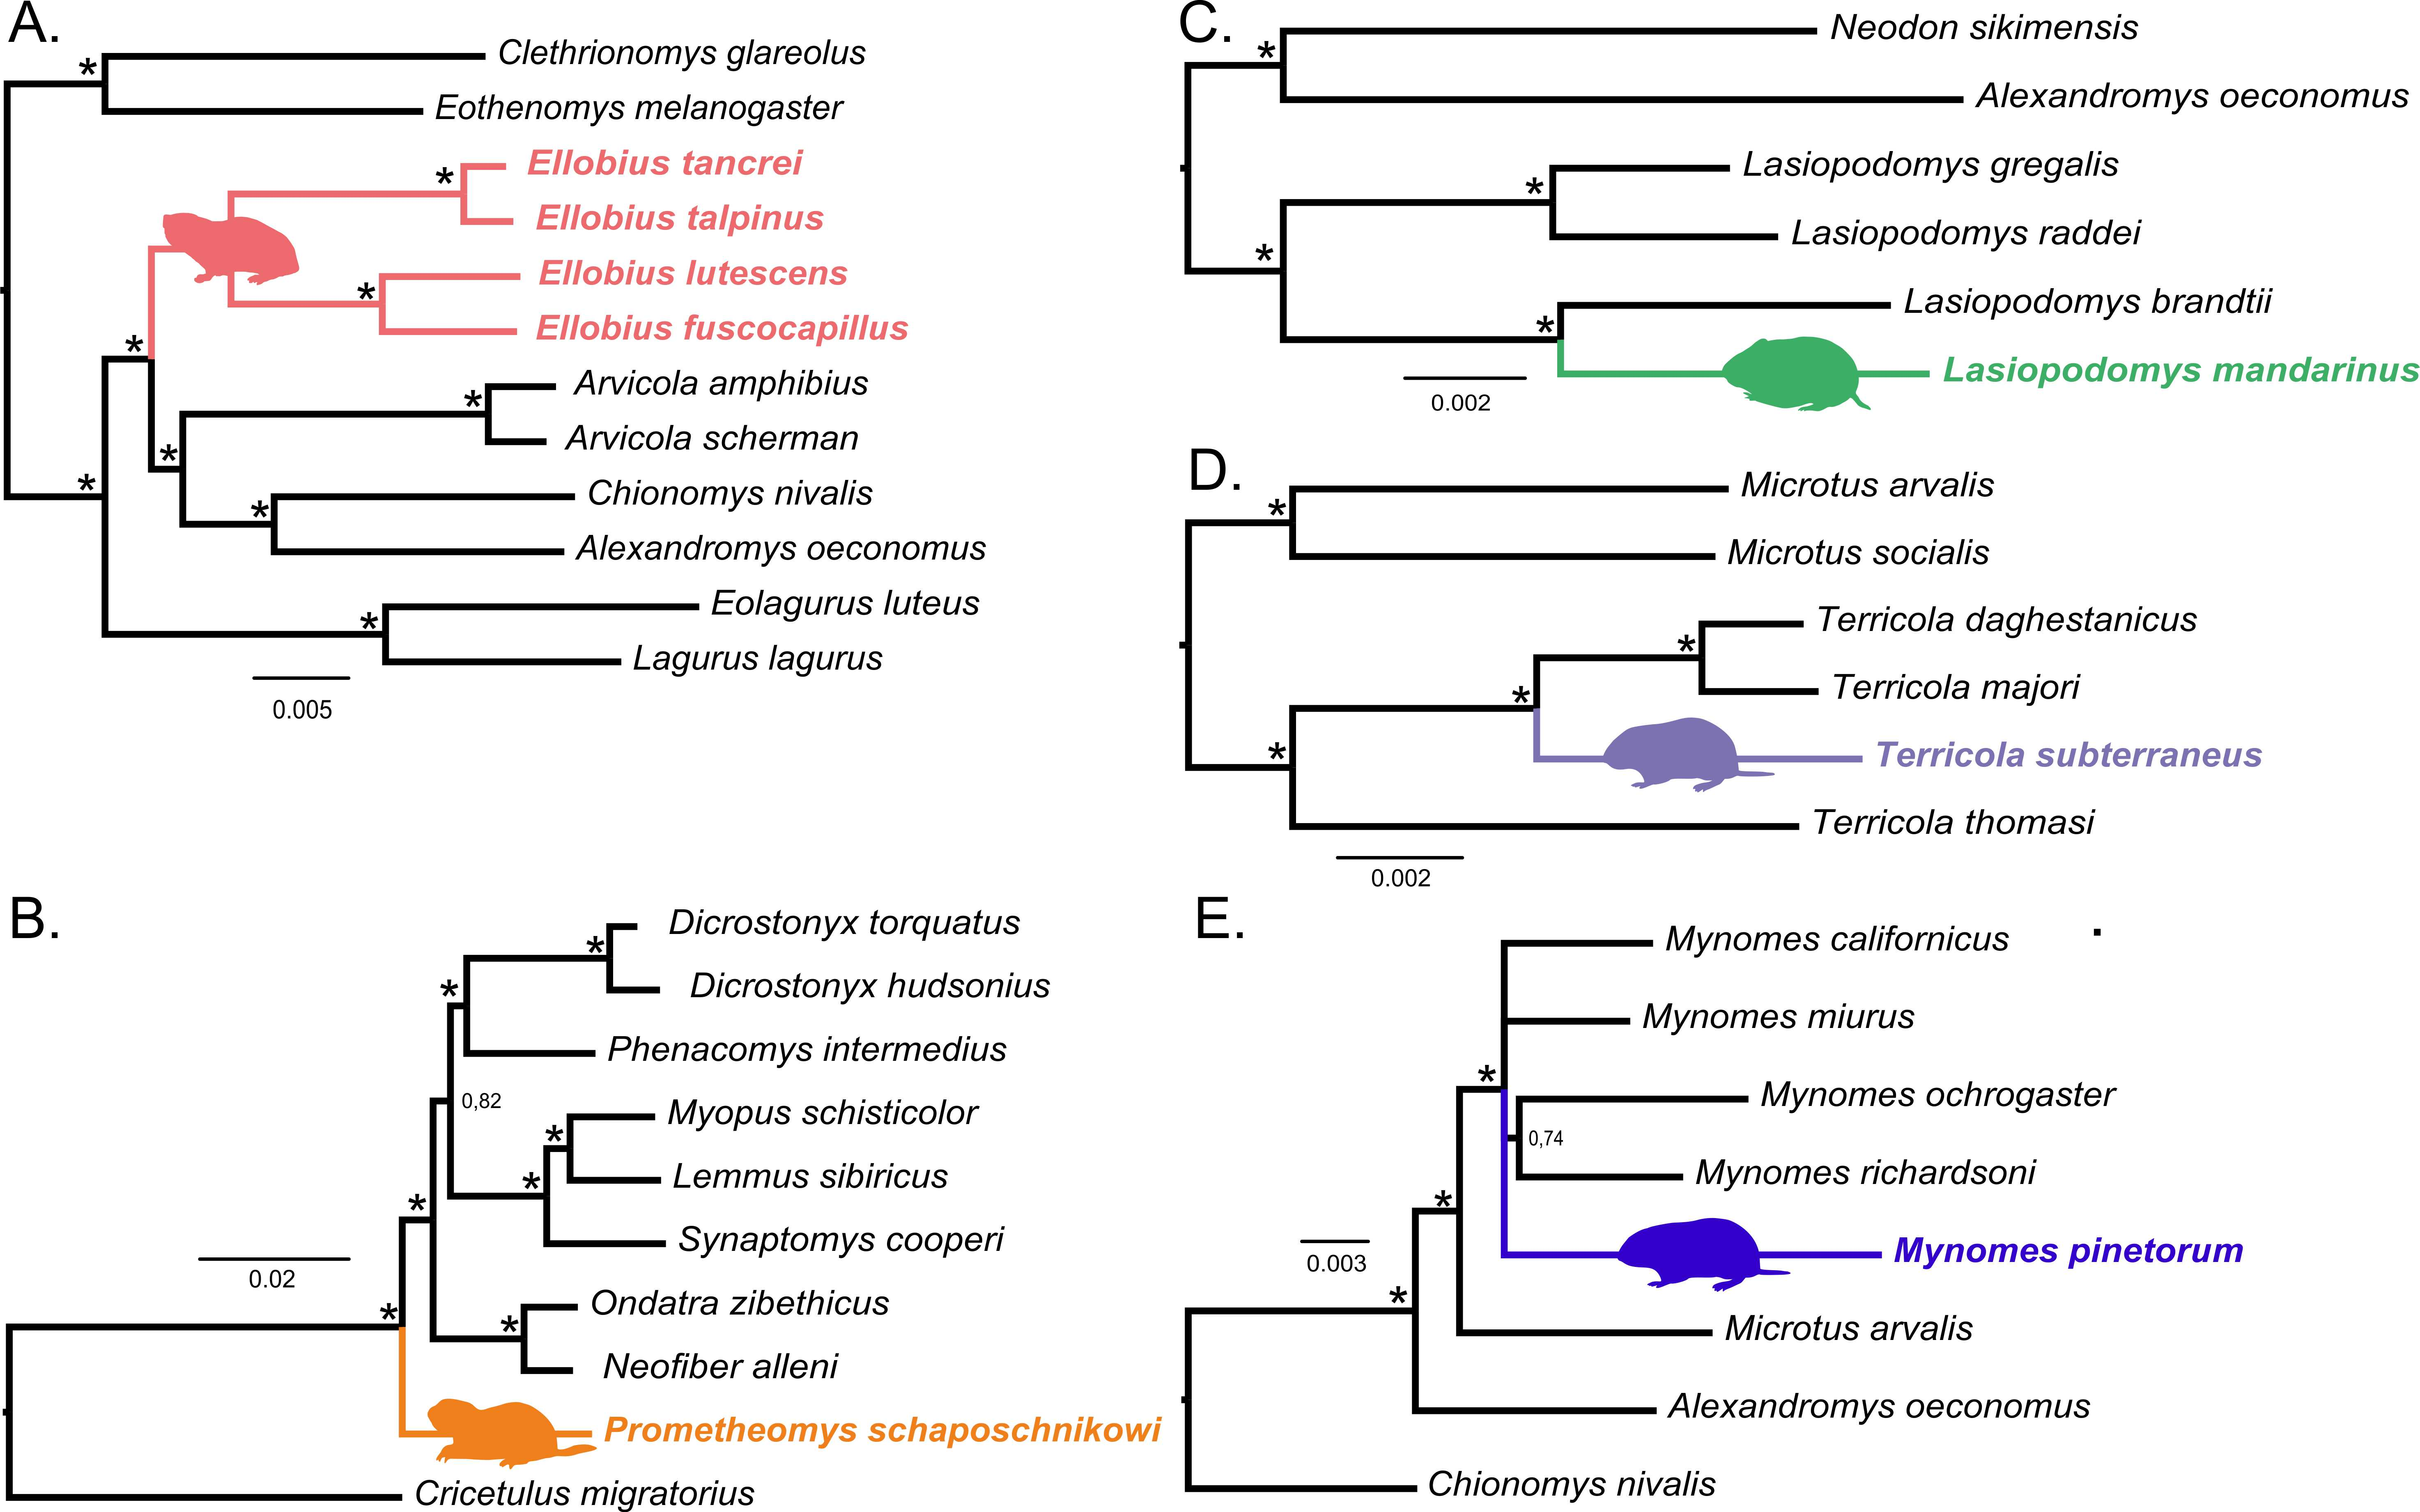
\includegraphics[width=\textwidth]{Cytb_separate_trees}
	\end{center}
	\caption{Филогенетические деревья, использованные для оценки отбора по отдельным ветвям. Подземные виды отмечены цветом. Звездочки (*) обозначают апостериорные байесовские вероятности 0,95 -- 1,0.} \label{Tree4Selection}
\end{figure}


 Достоверные отличия в значениях $\omega$ получены с использованием программы codeml для видов рода \textit{Ellobius}, \textit{Lasiopodomys mandarinus} и \textit{Terricola subterraneus}. Почти у всех подземных видов наблюдаются более высокие значения $\omega$ по сравнению наземными, за исключением \textit{T. subterraneus} (таблица \ref{PAMLtable}). Эта разница варьирует от одного (для \textit{Mymomes pinetorum}) до пяти раз для \textit{Lasiopodomys mandarinus}. Тесты сравнения с нейтральной моделью (b\_neut, таблица \ref{PAMLtable}) показали, что нуклеотидные последовательности гена \textit{CYTB} эволюционно не нейтральны у всех подземных грызунов. 

Анализ отбора алгоритмом aBSREL не показал свидетельств эпизодического отбора в анализируемой филогении. Результаты программы RELAX подтвердили изменения в уровне естественного отбора у подземных грызунов. Так, коэффициент отбора K для трех подземных представителей (\textit{Ellobius sp.}, \textit{L. mandarinus} и \textit{P. schaposchnikowi}; таблица \ref{Relax_cyt}) показал значения < 1, что может указывать на ослабление естественного отбора. В то же время, для представителей рода \textit{Ellobius} и для \textit{L. mandarinus} показаны повышенные значения $\omega$ при анализе отбора методом codeml. Значение K для \textit{T. subterraneus} намного превышало 1, что можно интерпретировать как то, что сила отбора увеличилась и коррелировала с более низким значением $\omega$ по сравнению с видами, обитающими на поверхности. Суммируя результаты этих анализов, можно сказать о наличии следов ослабления отбора в гене \textit{CYTB} у почти всех подземных грызунов.


\begin{table}[h!]
	\caption{Оценка $\omega$ с использованием branch model codeml. Fg --- foreground branch (подземные виды), Bg --- background branch (наземные виды). Подземные виды обозначены цветом на рисунке \ref{Tree4Selection}. b\_free --- модель независимого расчета по ветвям, b\_neut --- нейтральная модель. Достоверность сравнения типов моделей выражена в p.value, достоверные значения отмечены \textbf{жирным}.}\label{PAMLtable}
	\vspace{5mm}
	
\begin{center}
\begin{tabular}{|c|c|c|p{4.5cm}|p{4.5cm}|}
	\hline 
\textbf{Подземные виды} & \textbf{Fg} & \textbf{Bg} & \textbf{Сравнение моделей b\_free и M0} & \textbf{Сравнение моделей b\_free и b\_neut}\\ \hline
\textit{Ellobius sp.} & \textbf{0,0642} & \textbf{0,0243} & \textbf{2,33E-06} & \textbf{4,76E-81}\\ \hline
\textit{L. mandarinus} & \textbf{0,1325} & \textbf{0,0269} & \textbf{4,69E-05} & \textbf{0,00024}\\ \hline
\textit{M. pinetorum} & 0,0233 & 0,0224 & 0,9327 & \textbf{4,62E-24}\\ \hline
\textit{P. schaposchnikowi} & 0,0617 & 0,0356 & 0,0711 & \textbf{1,26E-09}\\ \hline
\textit{T. subterraneus} & \textbf{0,0071} & \textbf{0,0343} & \textbf{0,05} & \textbf{2,48E-17}\\ \hline
\end{tabular} 
\end{center}
\end{table}

\clearpage

\begin{table}[h!]
	\caption{Оценка уровеня отбора с использованием программы RELAX. K --- значение коэффициента отбора, P --- p-value, LRT --- likelihood ratio test. Подземные виды обозначены цветом на рисунке \ref{Tree4Selection}. Достоверные результаты отмечены \textbf{жирным}.}\label{Relax_cyt}
	\vspace{5mm}
	
\begin{center}
	\begin{tabular}{|c|l|l|l|}
		\hline
		\textbf{}                     & \multicolumn{3}{c|}{RELAX}              \\ \hline
		\textbf{Подземные виды} & \textbf{K}     & \textbf{P}     & \textbf{LRT}   \\ \hline
		\textit{Ellobius sp.}         & \textbf{0.52}  & \textbf{0}     & \textbf{23.97} \\ \hline
		\textit{L. mandarinus}        & \textbf{0}     & \textbf{0.001} & \textbf{11.78} \\ \hline
		\textit{M. pinetorum}         & 1.05           & 0.804          & 0.06           \\ \hline
		\textit{P. schaposchnikowi}   & \textbf{0.63}  & \textbf{0.023} & \textbf{5.15}  \\ \hline
		\textit{T. subterraneus}      & \textbf{23.22} & \textbf{0.014} & \textbf{6.02}  \\ \hline
	\end{tabular}
\end{center}
\end{table}

\subsection{Оценка частоты несинонимичных замен}

Мы рассчитали распределение замен в каждом сайте \textit{CYTB} отдельно и объединили по координатам доменов. Анализ по сайтам показал три позиции (таблица \ref{CytB_sites}) с достоверно более высокими значениями частоты несинонимичных замен в гене \textit{CYTB} у подземных видов: 4, 237 и 241. Кроме того, в позиции 236 достоверно повышена частота синонимичных замен. Сравнение распределение замен по целым доменам (таблица \ref{CytB_domains}, рис. \ref{Cyt_Dom_fig}) выявило значительные различия в мембранных доменах 1, 2, 5 и 9 и трансмембранных доменах 5 и 7 для несинонимичных замен (рис. \ref{Cyt_Dom_fig} A); и мембранный домен 6 и трансмембранный домен 5 для синонимичных замен (рис. \ref{Cyt_Dom_fig} B). 

\begin{table}[h!]
\caption{Сайты в гене \textit{CYTB} с достоверной разницей в частоте замен между подземными и наземными видами. NS -- несинонимичные замены, S -- синонимичные замены, Fs -- точный критерий Фишера, Holm -- значения p.value после поправки Холма-Бонферрони на множественные значения.}
\label{CytB_sites}
\vspace{5mm}

\begin{center}
\begin{tabular}{|c|c|c|c|c|c|}
	\hline 
\textbf{Тип замен} & \textbf{Позиция} & \textbf{Подземные} & \textbf{Наземные} & \textbf{Fs} & \textbf{Holm} \\ \hline 
NS & 4 & 0,875 & 0,1296 & 0,000049 & 0,023 \\ \hline 
NS & 237 & 0,75 & 0,07 & 0,000084 & 0,038 \\ \hline 
NS & 241 & 0,75 & 0,07 & 0,000084 & 0,039 \\ \hline 
S & 236 & 1 & 0,148 & 0,0000038 & 0,002 \\ \hline 
\end{tabular} 
\end{center}
\end{table}



\begin{table}[h!]
	\caption{Домены в гене \textit{CYTB} с достоверной разницей в частоте замен между подземными и наземными видами. NS -- несинонимичные замены, S -- синонимичные замены, Fs -- точный критерий Фишера, Holm -- значения p.value после поправки Холма-Бонферрони на множественное тестирование, Memb -- мембранный домен, TM -- трансмембранный домен.}\label{CytB_domains}
	\vspace{5mm}
\begin{center}	
	\begin{tabular}{|c|c|c|c|c|c|}
		\hline 
\textbf{Домены} & \textbf{Подземные} & \textbf{Наземные} & \textbf{Тип замен} & \textbf{Fs} & \textbf{Holm}\\ \hline 
Memb1 & 0,45 & 0,097 & NS & 0,00000033 & 0,000011\\ \hline 
Memb2 & 0,33 & 0,043 & NS & 0,00001176 & 0,000365\\ \hline 
Memb5 & 0,263 & 0,047 & NS & 0,00033176 & 0,008957\\ \hline 
Memb9 & 0,52 & 0,15 & NS & 0,00005434 & 0,001522\\ \hline 
TM5 & 0,64 & 0,10 & NS & 0,00000001 & 0,000000\\ \hline 
TM7 & 0,29 & 0,06 & NS & 0,00004166 & 0,001208\\ \hline 
Memb6 & 0,40 & 0,19 & S & 0,00000012 & 0,000004\\ \hline 
TM5 & 0,42 & 0,19 & S & 0,00002733 & 0,000820 \\ \hline
	\end{tabular} 
\end{center}
	
\end{table}

\begin{figure}[h!]
	\begin{center}
		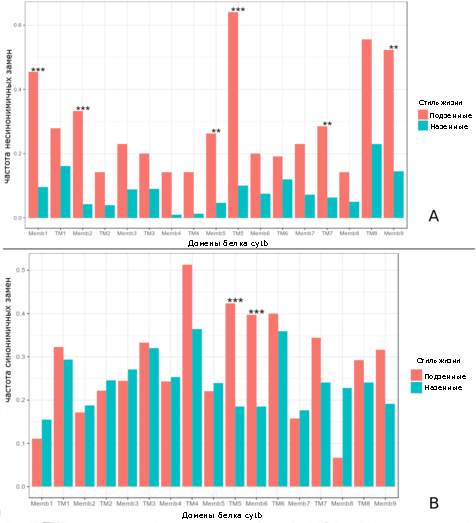
\includegraphics[width=0.7\textwidth]{cyt_domains}
	\end{center}
	\caption{Частоты распределения несинонимичных (A) и синонимичных (B) замен по доменам гена \textit{CYTB} у подземных и назменых грызунов. Достоверные различия между частотами обозначены звездочками(*): * -- p.value < 0.05, ** -- p.value < 0.01, *** -- p.value < 0.001 }\label{Cyt_Dom_fig}
\end{figure}

%\textit{Добавить рисунок структуры доменов}

\clearpage

\section{Поиск следов отбора в митохондриальных геномах}

\subsection{Характеристика собранных митохондриальных геномов}

Всего в лаборатории эволюционной геномики и палеогеномики ЗИН РАН было собрано 34 новых митохондриальных генома представителей Arvicolinae (таблица \ref{mt_stats}). Все собранные последовательности, а также доступные в базе данных NCBI, были использованы для реконструкции филогении подсемейства.


%Наземные виды: \textit{Ondatra zibethicus} Linnaeus, 1766; \textit{Dicrostonyx torquatus} Pallas, 1778; \textit{Myopus schisticolor} Lilljeborg, 1844; \textit{Lemmus sibiricus} Kerr, 1792; \textit{Alticola tuvinicus} Ognev, 1950; \textit{Alticola strelzovi} Kastsch, 1899; \textit{Craseomys rufocanus} Sundevall, 1846; \textit{Craseomys regulus} Thomas, 1906; \textit{Clethrionomys glareolus} Schreber, 1780; \textit{Lasiopodomys brandtii} Radde, 1861; \textit{Lasiopodomys gregalis} Pallas, 1779; \textit{Alexandromys fortis} Büchner, 1889; \textit{Chionomys nivalis} Martins, 1842; \textit{Chionomys gud} Satunin, 1909; \textit{Lagurus lagurus} Pallas, 1773; \textit{Eolagurus luteus} Eversmann, 1840; \textit{Microtus californicus} Peale, 1848; \textit{Microtus longicaudus} Merriam, 1888; \textit{Microtus arvalis} Pallas, 1778; \textit{Microtus socialis} Pallas, 1773; \textit{Terricola daghestanicus} Shidlovsky, 1919.

%Подземные виды: \textit{Prometheomys shchaposhnikowi}, \textit{Lasiopodomys mandarinus}, \textit{Ellobius} (4 вида), \textit{Terriocola subterraneus}, \textit{Hyperacrius fertilis} True, 1894.

Отдельной задачей была проверка качества ридов для \textit{Hyperacrius fertilis} из-за древности образца (1903 г.). Молекуляное изучение музейных коллекций требует множества дополнительных проверок качества сырых прочтений. Прежде всего, из-за проблемы дезаминирования, которая возникает в виде включения тимина вместо цитозина (C-to-T) на 5'-концах и аденина вместо гуанина (G-to-A) на 3'-концах последовательности. Анализ mapDamage показал низкое значение дезаминирования (рис. \ref{MapDamage}). Неправильное включение тимина вместо цитозина (красный) варьировалось от 12.09 \% до 17.94 \%, аденина вместо гуанина (синий) -- от 12.84 \% до 17.49 \%. Уровни ошибочного включения сравнимы со всеми другими вариантами замен, окрашенными в серый цвет, а также аналогичными значениям из статей (\cite{Molto2017}).


\begin{figure}[h!]
	\begin{center}
		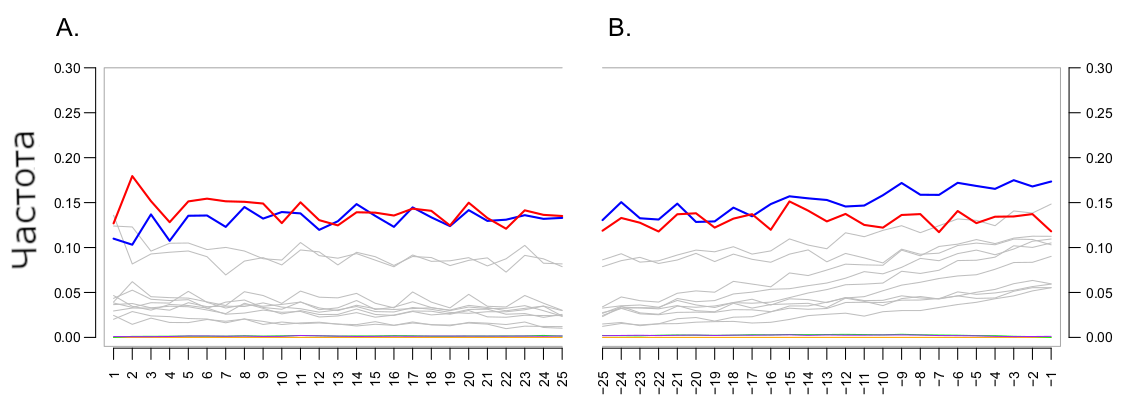
\includegraphics[width=\textwidth]{MapDamage Hyper}
	\end{center}
	\caption{Дезаминирование нуклеотидов на 5` (А) и 3` конце (В), рассчитанные с использованием MapDamage. Все варианты замен отмечены серым, кроме замены гуанина на аденин (G>A, голубой цвет) и цитозина на тимин (C>T, красный цвет)}\label{MapDamage}
\end{figure}


Собранные митогеномы представляют собой кольцевые двуцепочечные последовательности ДНК (рис. \ref{mitogenome}). Состав и порядок генов всех последовательностей соответствует структуре митохондриального генома других млекопитающих: 13 белок-кодирующих генов, 22 транспортные РНК (тРНК), две рибосомные РНК (рРНК) и некодирующая регуляторная область (D-петля). Девять генов (\textit{ND6} и 8 тРНК) были ориентированы в обратном (reverse) направлении, тогда как остальные транскрибировались в прямом. Нами не было обнаружено каких-либо структурных изменений в порядке генов или их количестве, которые отличали бы подземных грызунов от наземных сестринских видов.

\begin{figure}[h!]
	\begin{center}
		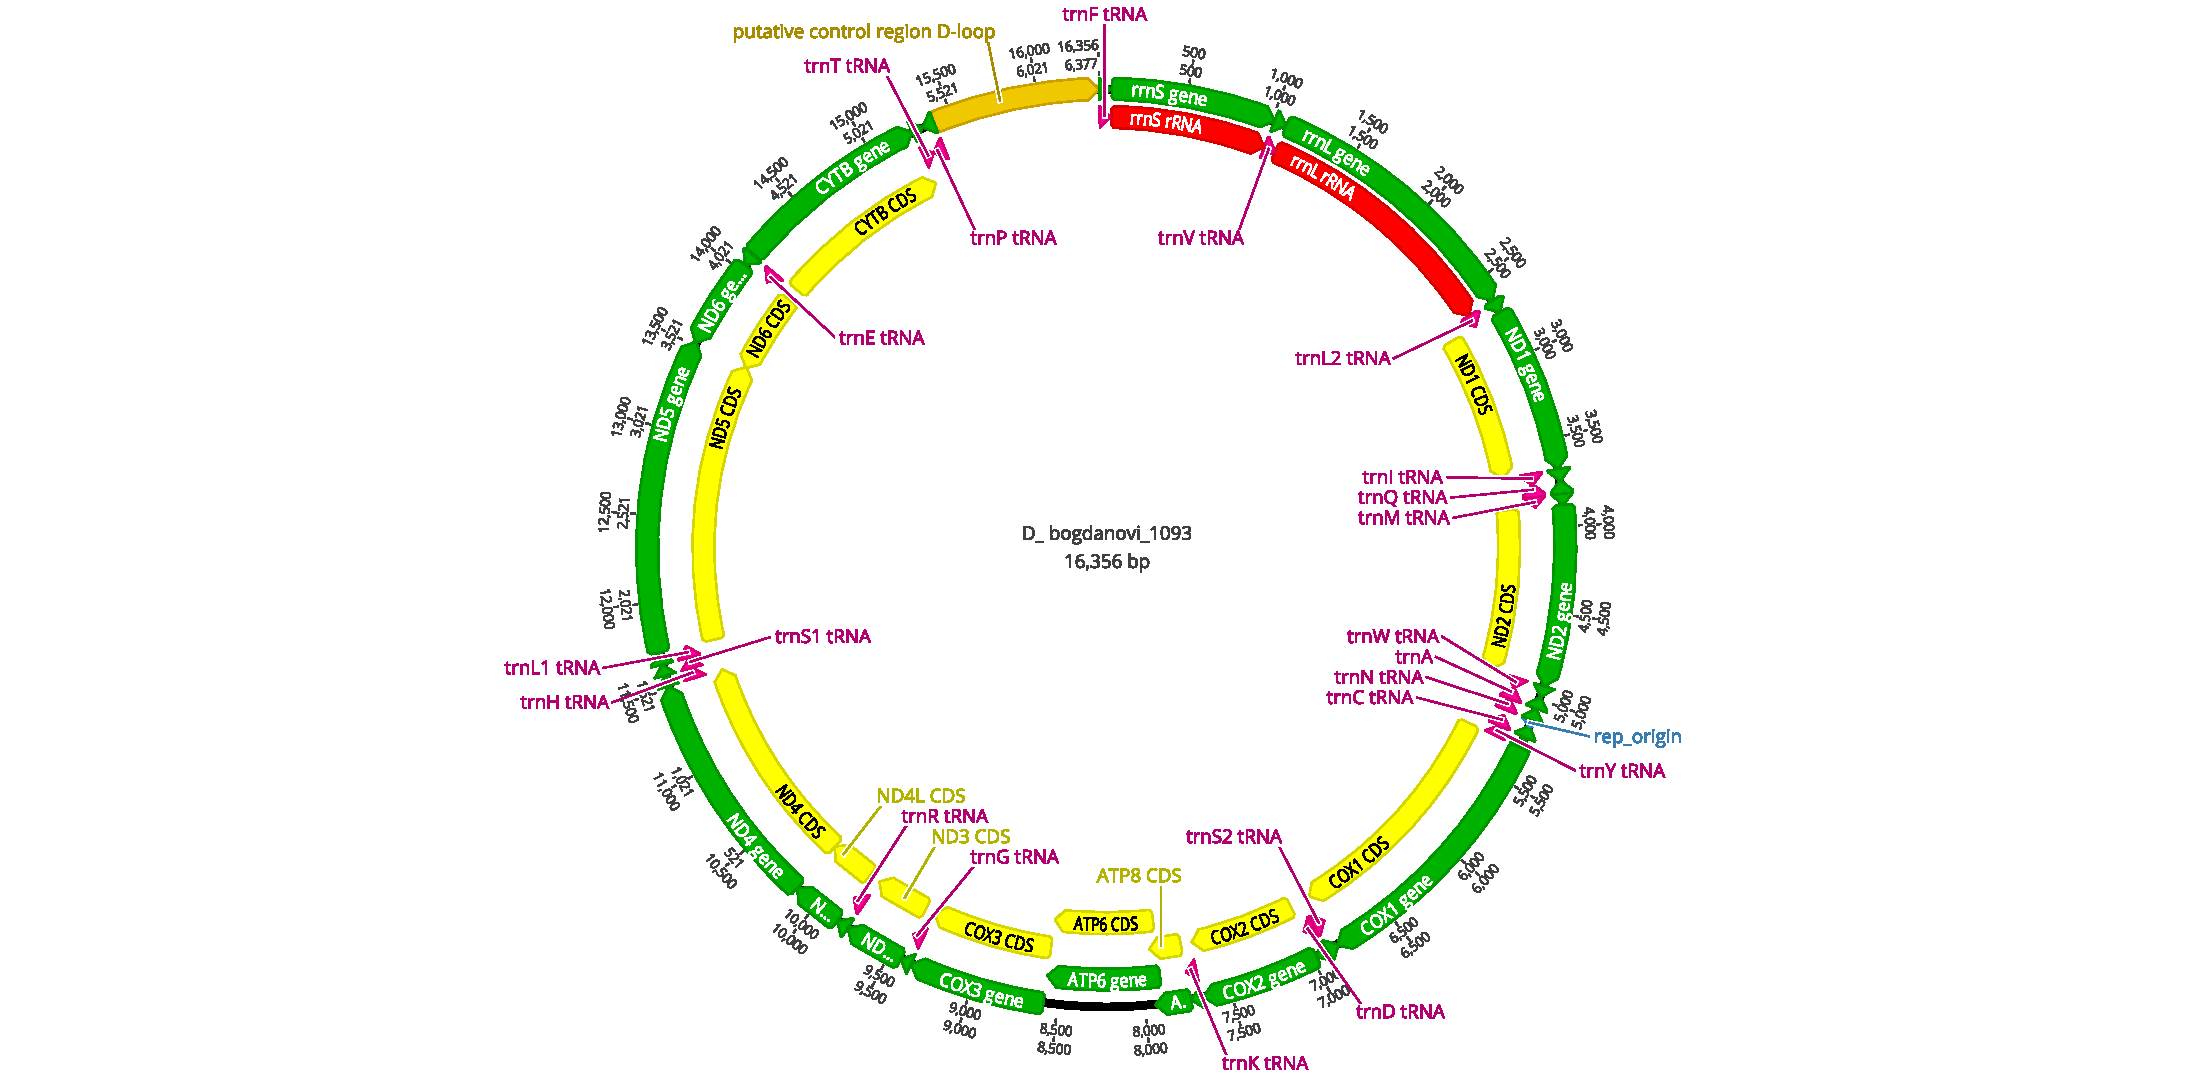
\includegraphics[width=\textwidth]{Dinaromys_mitogenome}
	\end{center}
	\caption{Собранный митохондриальный геном \textit{Dinaromys bogdanovi} Martino, 1922. Зеленым отмечены гены, желтым -- CDS, красным -- рРНК, розовым -- тРНК}\label{mitogenome}
\end{figure}

Филогенетическая реконструкция (рис. \ref{Tree_13_genes}) с использованием митохондриальных геномов полевочьих на полноценной выборке таксонов в целом не противоречит предыдущим данным Абрамсон Н.И. с соавторами (\cite{Abramson2009}). Для дальнейшего изучения конвергентной эволюции подземных грызунов мы взяли выборочные наборы таксонов, позволяющие составить полноценные группы сравнения для подземных видов (отмечены на рисунке \ref{tree_mito}). 

\begin{figure}[h!]
\begin{center}
	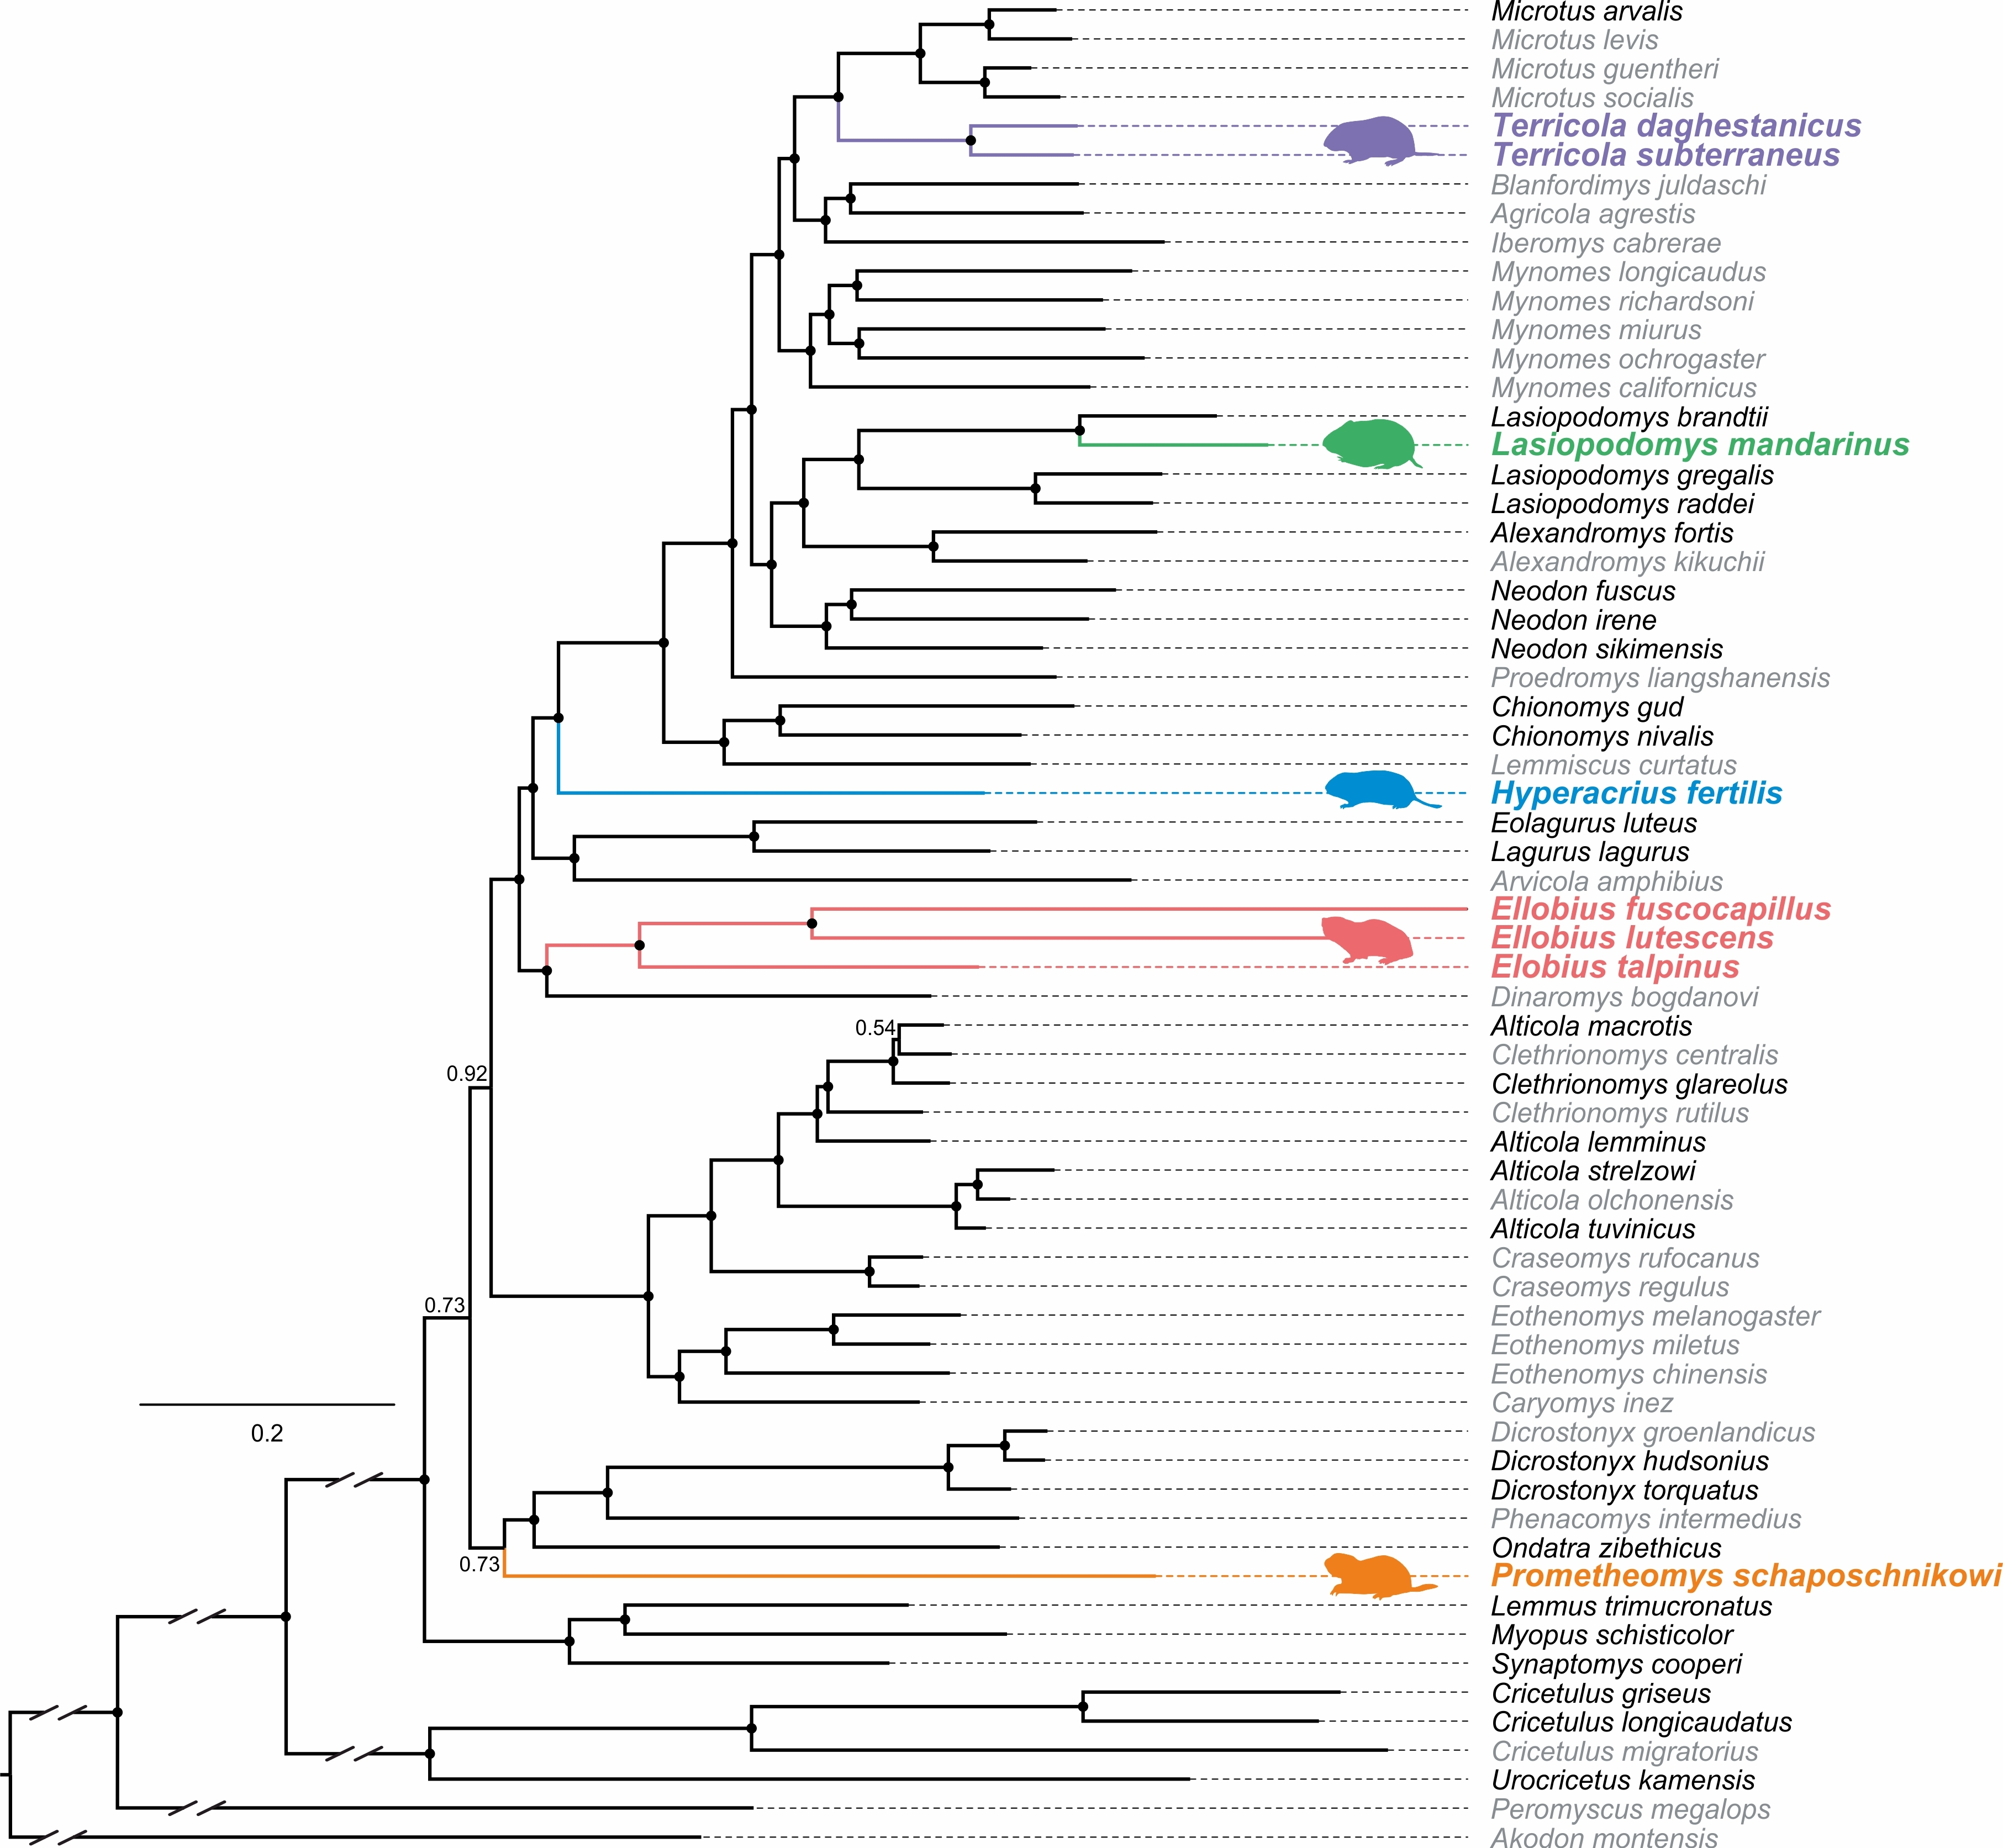
\includegraphics[width=\textwidth]{main_tree_mito_col}
\end{center}
	\caption{Филогенетическое дерево, построенное по последовательности 13 белок-кодирующих генов. Подземные виды обозначены цветом.}
	\label{Tree_13_genes}
\end{figure}


Для начала мы сравнили митохондриальные геномы по GC-обогащенности и смещению нуклеотидов в паре GC (GC-skew). Результаты сравнения показали увеличение среднего значения \% GC и уменьшение GC-skew. Разница в различиях оказалась недостоверная (рис. \ref{boxplot_GC_GSskew}). 

\begin{figure}[h!]
\begin{center}
	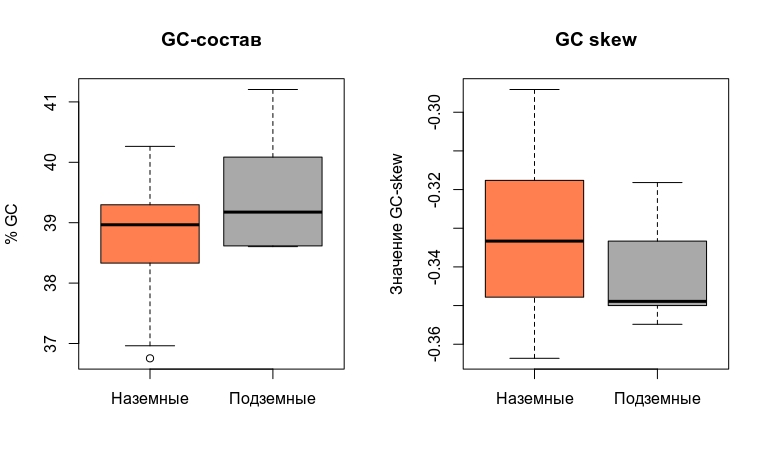
\includegraphics[width=0.7\textwidth]{GC genomes}
\end{center}
\caption{Сравнение \% GC и GC-skew у подземных и наземных видов}\label{boxplot_GC_GSskew}
\end{figure}


\subsection{Анализ частоты несинонимичных замен}

Доля несинонимичных замен в митохондриальных геномах подземных грызунов достоверно выше, чем у наземных, при подсчете количества замен, нормировав их на количество взятых в анализ видов (рис. \ref{boxplot_NS}). При оценке частот замен по каждому белок-кодирующему гену в отдельности тенденция повторяется --- в каждом гене доля несинонимичных замен достоверно выше у подземных грызунов, чем у наземных (рис. \ref{manhattan_NS}).

\begin{figure}[h!]
\begin{center}
	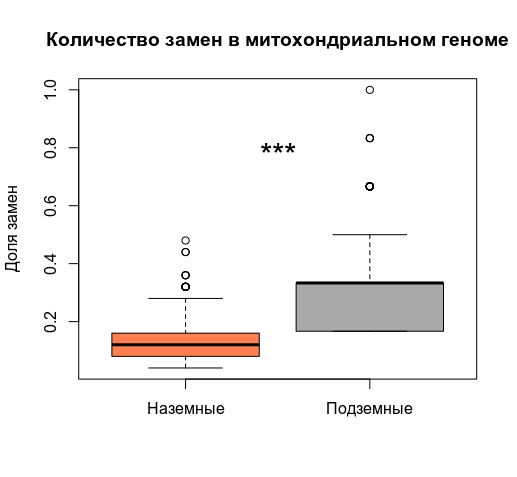
\includegraphics[width=0.6\textwidth]{Subst_all_boxplot}
\end{center}
	\caption{Соотношение несинонимичных замен у наземных и подземных грызунов}\label{boxplot_NS}
\end{figure}


\begin{figure}[h!]
	\begin{center}
		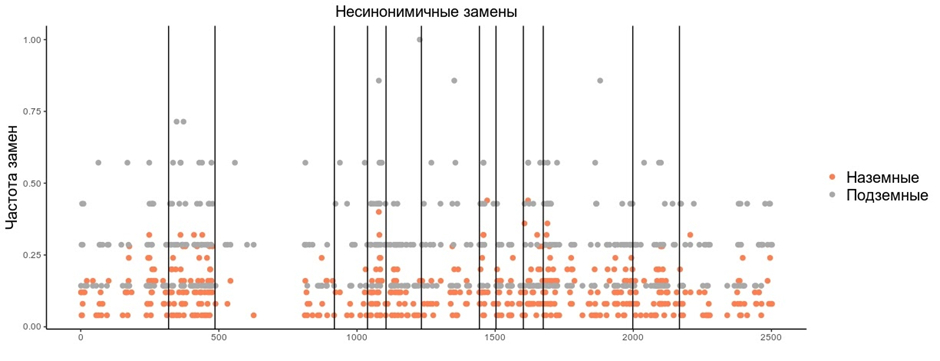
\includegraphics[width=0.9\textwidth]{Distribution_mitogenomes}
	\end{center}
	\caption{Распределение несинонимичных замен по белок-кодирующим генам у подземных и наземных грызунов.}\label{manhattan_NS}
\end{figure}

%Таблица со значениями для каждого гена частоты

\subsection{Поиск параллельных аминокислотных замен}

Мы, по аналогии с логикой исследования гена \textit{CYTB}, искали характерные только для подземных грызунов замены. При анализе белок-кодирующих митохондриальных генов были выявлены параллельные замены в генах \textit{COX1, COX3, ND5, ND6} и \textit{CYTB} (таблица \ref{Underground_subs}). Больше всего замен было обнаружено в гене \textit{CYTB}. При дальнейшей проверке оказалось, что все эти замены не достоверные.

\begin{table}[h!]
	\caption{Обнаруженные параллельные аминокислотные замены у подземных грызунов}\label{Underground_subs}
	\vspace{5mm}
\begin{tabular}{|l|c|c|c|c|c|c|}
	\hline
	& \textit{COX1} & \textit{COX3} & \textit{ND5} & \multicolumn{3}{c|}{\textit{CYTB}} \\ \hline
	Вид   / позиция              & 73   & 121  & 466 & 56      & 338    & 357    \\ \hline
	Наземные виды                & Met  & Ile  & Phe & Thr     & Ile    & Ala    \\ \hline
	\textit{Ellobius lutescens}          & Val  & --   & --  & Ser     & Val    & --     \\ \hline
	\textit{Ellobius fuscocapillus}       & Ile  & --   & Leu & --      & --     & Thr    \\ \hline
	\textit{Ellobius talpinus}            & --   & Val  & Leu & --      & Val    & --     \\ \hline
	\textit{Prometheomys schaposchnikowi} & Ile  & Val  & --  & Ser     & --     & Thr    \\ \hline
	\textit{Lasiopodomys mandarinus}      & Ile  & --   & --  & Ser     & Val    & Thr    \\ \hline
	\textit{Hyperacrius fertilis}         & --   & Val  & --  & --      & --     & --     \\ \hline
	\textit{Terricola subterraneus}       & --   & --   & Leu & --      & --     & --     \\ \hline
\end{tabular}	
\end{table}


\subsection{Оценка уровня и направления отбора}

Уровень и направление отбора на белок-кодирующих генах оценивали несколькими способами: отдельно по каждому подземному виду (или нескольким в случае рода \textit{Ellobius}), сравнивая его только с филогенетически близкими наземными видами (рис. \ref{tree_mito}) подходами REXAL, aBSREL и codeml. Из-за базального положения \textit{P. schaposchnikowi} уровень отбора оценивали дважды, сравнивания его с хомяками и с другими представителями <<первой>> радиации.   

\begin{figure}[h!]
	\begin{center}
		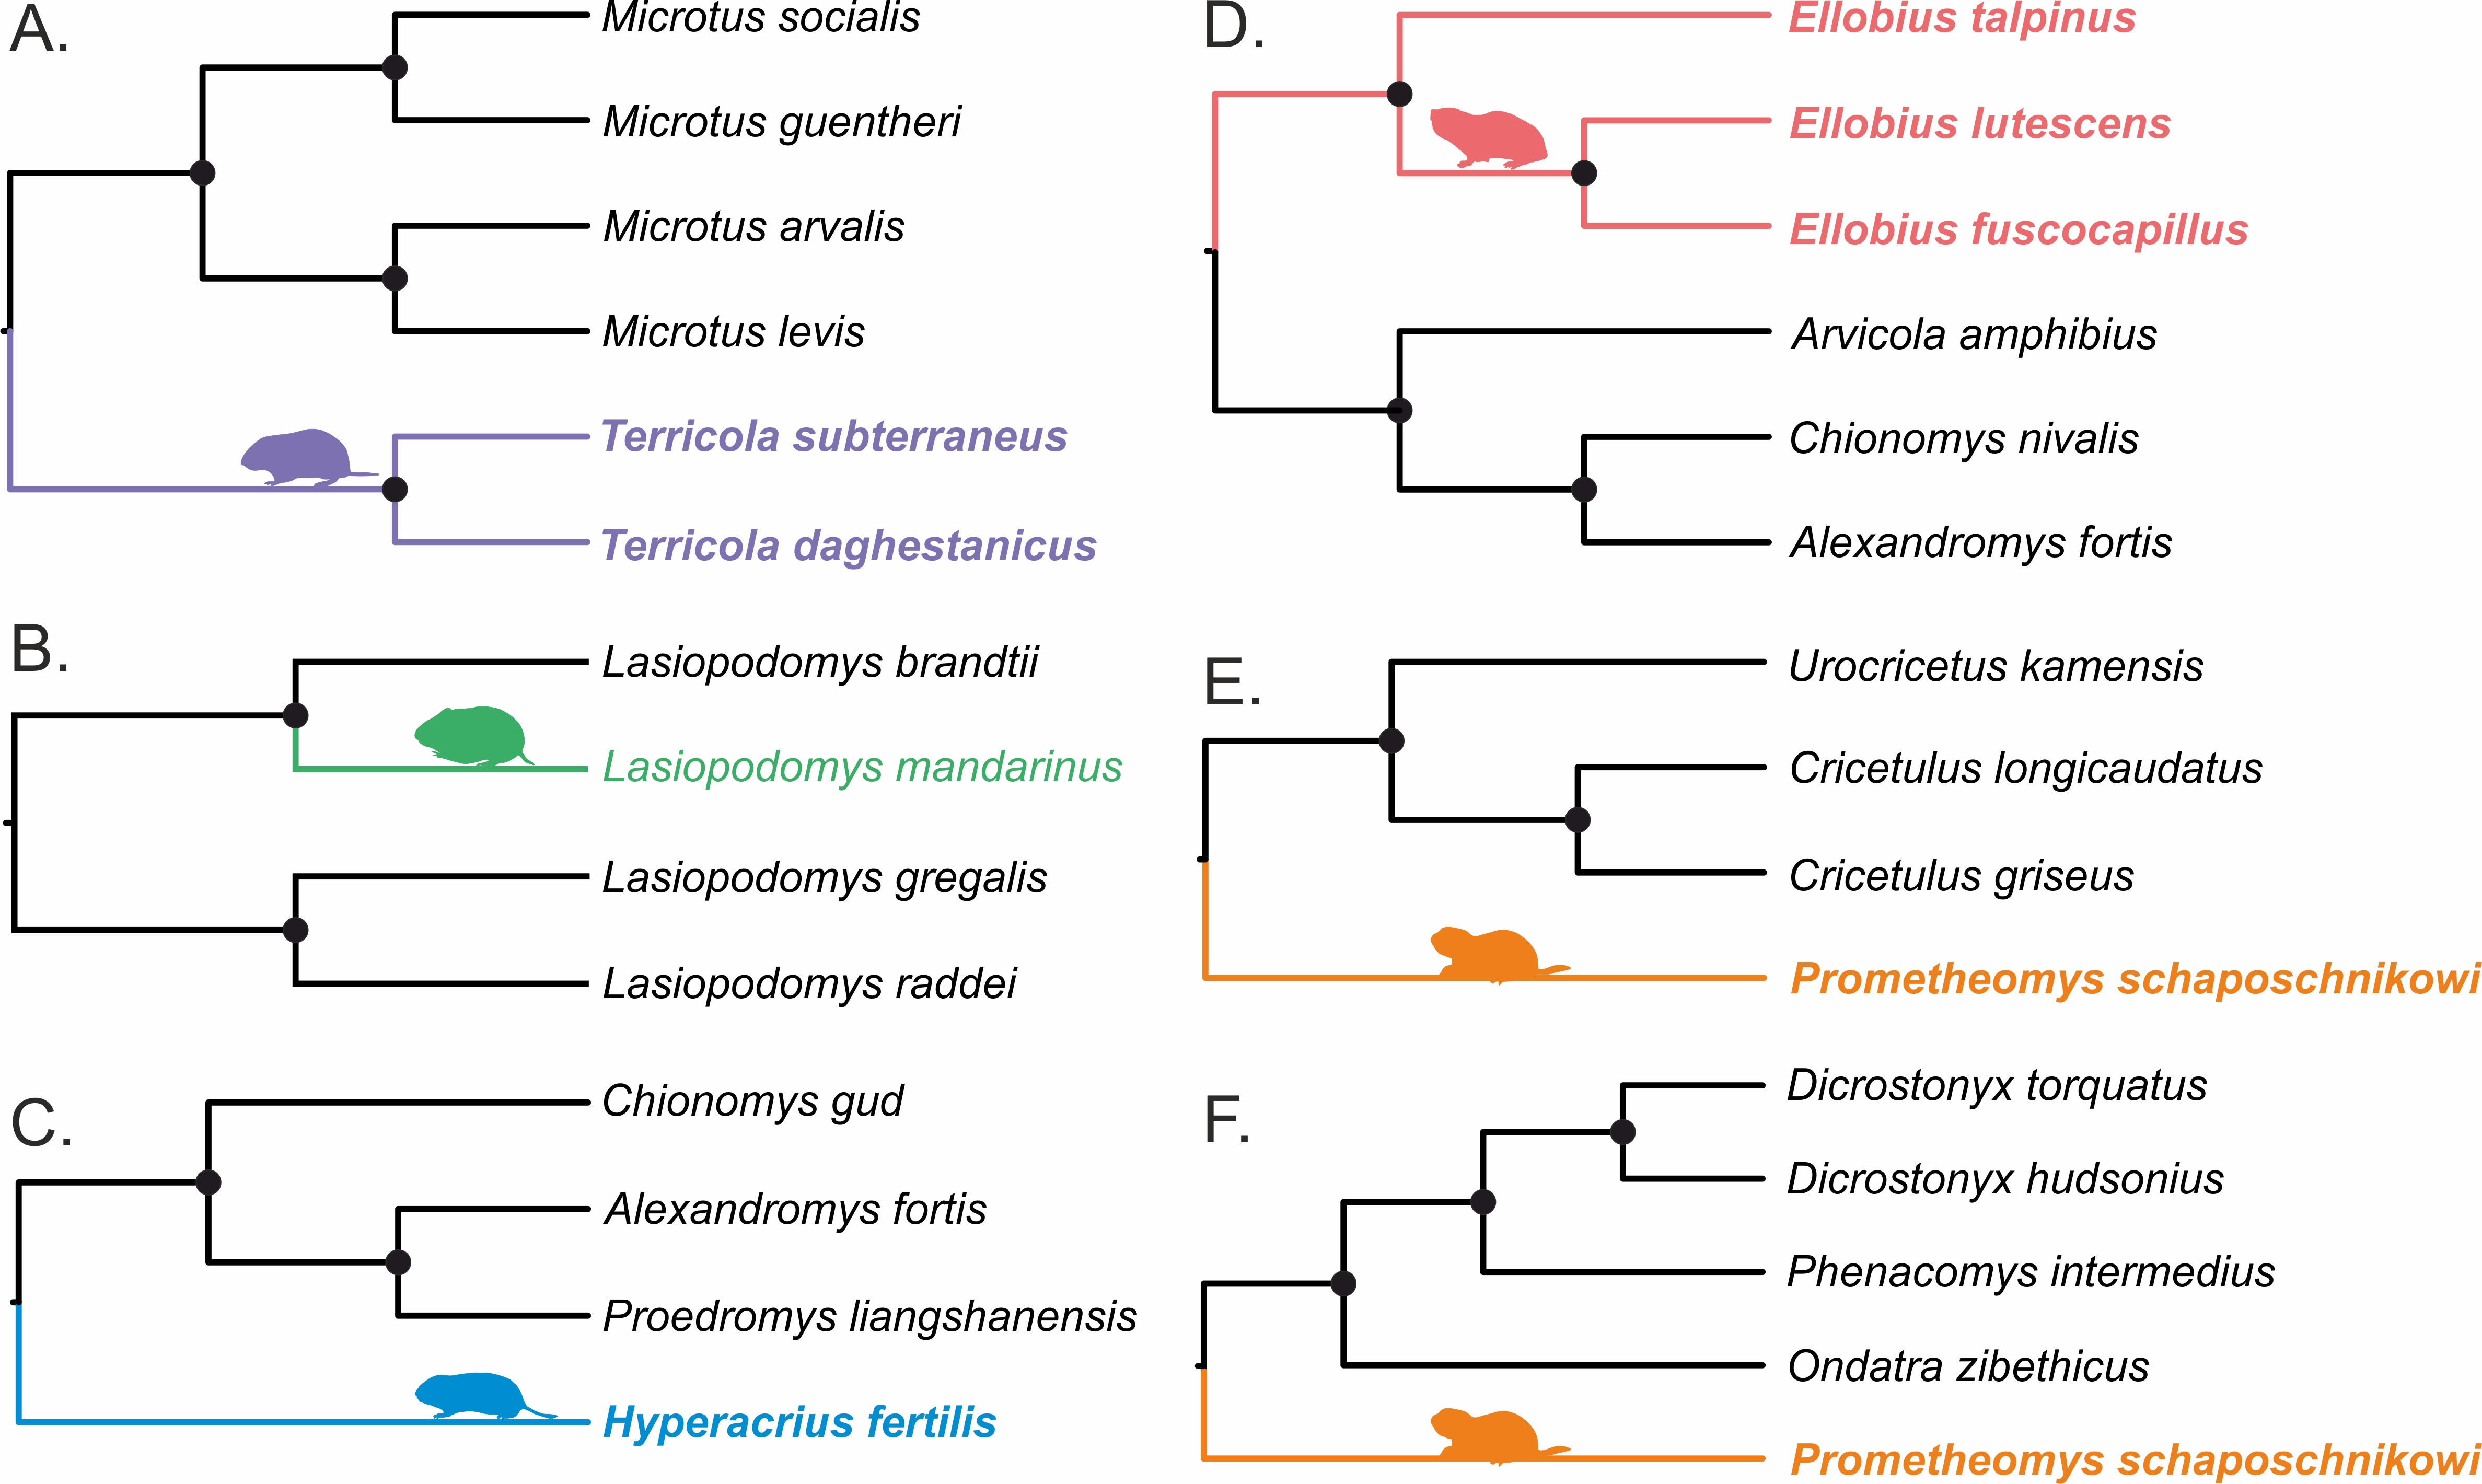
\includegraphics[width=\textwidth]{separate_mito_col}
	\end{center}
	\caption{Филогенетические деревья, использованные для оценки отбора по отдельным ветвям. Подземные виды обозначены цветом. Для каждого подземного вида или группы видов использовались филогенетически близкие наземные таксоны.}
	\label{tree_mito}
\end{figure}


Для каждого из подземных грызунов мы провели сравнение по каждому митохондриальному гену (таблица \ref{MT_branch}) методом codeml. У представителей рода \textit{Ellobius} разница в отборе наблюдается во всех митохондриальных генах, кроме \textit{ND2,3,5,6} и \textit{COX3}. Несколько генов под отбором обнаружено также у \textit{L. mandarinus}: \textit{COX3} и \textit{CYTB}. Только один ген с достоверной разницей в уровне отбора найден для \textit{P. schaposchnikowi} --- \textit{COX3}. У оставшихся представителей подземных грызунов не обнаружено генов с достоверным отличием от наземных видов. Значимые различия наблюдались в последовательностях \textit{COX3} и \textit{CYTB} для двух подземных видов одновременно: в \textit{COX3} для \textit{P. schaposchnikowi} и \textit{L. mandarinus} и в \textit{CYTB} для \textit{L. mandarinus} и представителей рода \textit{Ellobius}. 
Хотя значения $\omega$ существенно различались в зависимости от генов и анализируемых видов, в любом случае значение $\omega$ не превышало единицы. Однако все достоверно различающиеся значения $\omega$ были выше для подземных видов, чем для наземных. 

\begin{landscape}
	
	\begin{table}[]
		\caption{Оценка уровня отбора независимо у всех филогенетических линий подземных грызунов методом codeml. \textbf{Жирным} обозначены достоверные различия между подземными и наземными видами после поравки на множественное сравнение. Fg --- foreground branch (подземные виды), Bg --- background branch (наземные виды). Ветви обозначены цветом на рисунке \ref{tree_mito}. NA -- рассчитать значение невозможно. }\label{MT_branch} \vspace{5mm}
		\large
		
		\begin{tabular}{|c|c|c|c|c|c|c|c|c|c|c|c|c|}
			\hline
			\multicolumn{1}{|l|}{}    & \multicolumn{2}{l|}{\textit{Ellobius sp.}} & \multicolumn{2}{p{5cm}|}{\textit{P. schaposchnikowi VS хомяки}} & \multicolumn{2}{p{5cm}|}{\textit{P. schaposchnikowi VS первая радиация}} & \multicolumn{2}{l|}{\textit{L. mandarinus}} & \multicolumn{2}{l|}{\textit{H. fertilis}} & \multicolumn{2}{l|}{\textit{Terricola}} \\ \hline
			\multicolumn{1}{|l|}{Ген} & fg & bg & fg & bg & fg & bg & fg & bg & fg & bg & fg & bg \\ \hline
			{\textit{ATP6}} & \textbf{0.132} & \textbf{0.039} & NA & 0.015 & NA & 0.034 & 0.138 & 0.075 & NA & 0.022 & 0.042 & 0.030 \\ \hline
			\textit{ATP8} & \textbf{0.739} & \textbf{0.163} & 0.903 & 0.153 & 0.376 & 0.269 & 0.184 & 0.240 & NA & 0.198 & 0.095& 0.079 \\ \hline
			\textit{COX1} & \textbf{0.033} & \textbf{0.009} & 0.138 & 0.008 & 0.029 & 0.010 & 0.036 & 0.023 & NA & 0.007 & 0.002& 0.027 \\ \hline
			\textit{COX2} & \textbf{0.217} & \textbf{0.022} & NA & 0.006 & 0.023 & 0.029 & 0.108 & 0.039 & NA & 0.018 & 0.030& 0.029 \\ \hline
			\textit{COX3} & 0.087 & 0.044 & \textbf{0.051} & \textbf{0.012} & 0.055 & 0.019 & \textbf{0.117} & \textbf{0.028} & NA & 0.033 & 0.028& 0.041 \\ \hline
			\textit{CYTB} & \textbf{0.060} & \textbf{0.021} & 0.048 & 0.021 & 0.050 & 0.028 & \textbf{0.234} & \textbf{0.028} & NA & 0.021 & 0.017& 0.030 \\ \hline
			\textit{ND1} & \textbf{0.064} & \textbf{0.029} & 0.042 & 0.030 & 0.059 & 0.021 & 0.075 & 0.020 & 0.009 & 0.027 & 0.011& 0.035 \\ \hline
			{\textit{ND2}} & 0.133 & 0.084 & NA & 0.048 & NA & 0.085 & 0.198 & 0.085 & NA & 0.076 & 0.104& 0.092 \\ \hline
			\textit{ND3} & 0.119 & 0.057 & 0.063 & 0.027 & NA & 0.067 & 0.234 & 0.116 & NA & 0.019 & 0.079& 0.094 \\ \hline
			\textit{ND4} & \textbf{0.095} & \textbf{0.045} & 0.045 & 0.031 & 0.095 & 0.057 & 0.165 & 0.072 & 0.107 & 0.051 & 0.035& 0.075 \\ \hline
			\textit{ND4l} & \textbf{0.179} & \textbf{0.038} & 0.009 & 0.017 & NA & 0.101 & 0.100 & 0.073 & NA & 0.036 & 0.000& 0.083 \\ \hline
			{\textit{ND5}} & 0.098 & 0.069 & 0.071 & 0.037 & NA & 0.052 & 0.179 & 0.068 & NA & 0.062 & 0.093& 0.055 \\ \hline
			\textit{ND6} & 0.149 & 0.084 & NA & 0.052 & 0.681 & 0.045 & 0.054 & 0.121 & NA & 0.104 & 0.013& 0.046 \\ \hline
			
		\end{tabular}
	\end{table}

\end{landscape}

Используя алгоритм aBSREL, мы обнаружили следы эпизодического положительного отбора в гене \textit{COX2} для \textit{E. lutescens} и в двух генах \textit{P. schaposchnikowi}: \textit{ATP8} при сравнении с видами Arvicolinae и \textit{ND5} при сравнении с хомяками (таблица \ref{MT_absrel}).

\begin{table}[]
	\caption{Оценка уровня отбора независимо для всех филогенетических линий подземных грызунов методом absrel. Подземные виды обозначены цветом на рисунке \ref{tree_mito}. B -- длина ветви; LRT -- Likelihood-ratio test; NA -- рассчитать значение невозможно. }\label{MT_absrel} \vspace{5mm}
	
	\begin{tabular}{|p{4cm}|p{3.5cm}|l|l|p{1.5cm}|p{3.5cm}|}
		\hline
		\textbf{Группа сравнения} & \textbf{Вид} & \textbf{B} & \textbf{LRT} & \textbf{P.value} & \textbf{Распределене ω по сайтам} \\ \hline
		\textit{Ellobius} & \textit{E. lutescens} & 0.0072 & 17.9838 & 0.0001 & \begin{tabular}[c]{@{}l@{}}ω1 = 0.238 (81\%)\\ ω2 = 15.4 (19\%)\end{tabular} \\ \hline
		\textit{P. schaposchnikowi} \& первая радиация & \textit{P. schaposchnikowi} & 0.0149 & 4.4686 & 0.0390 & \begin{tabular}[c]{@{}l@{}}ω1 = 0.395 (89\%)\\ ω2 = 16.7 (11\%)\end{tabular} \\ \hline
		\textit{P. schaposchnikowi} \& \textit{Cricetulus sp.} & \textit{P. schaposchnikowi} & 0.1443 & 6.0817 & 0.0171 & \begin{tabular}[c]{@{}l@{}}ω1 = 0.0553 (90\%)\\ ω2 = NA (10\%)\end{tabular} \\ \hline
	\end{tabular}
\end{table}

Анализ RELAX подтвердил изменения в уровне отбора подземных грызунов (таблица \ref{MT_relax}) по сравнению с наземными грызунами. Так, мы обнаружили несколько генов с K-значениями < 1 для представителей рода \textit{Ellobius}, \textit{L. mandarinus} и \textit{P. schaposchnikowi}. Семь генов для \textit{Ellobius}: \textit{ATP6}, \textit{COX1}, \textit{COX3}, \textit{CYTB}, \textit{ND1}, \textit{ND2} и \textit{ND4} и столько же для \textit{P. schaposchnikowi} при сравнении с <<первой радиацией>> Arvicolinae: \textit{COX1}, \textit{COX3}, \textit{ND2}, \textit{ND4} и \textit{ND5} продемонстрировали достоверное ослабление отбора. Ген \textit{COX3} \textit{P. schaposchnikowi} также достоверно отличается от видов \textit{Cricetulus} по этому признаку. Список генов \textit{L. mandarinus} более скромен и включает всего три: \textit{COX1}, \textit{COX3} и \textit{CYTB}. У оставшихся подземных грызунов: \textit{H.fertilis} и двух видов рода \textit{Terricola} гены с достоверным ослаблением или усилением отбора не обнаружены.
Многие гены выявлены у нескольких подземных видов одновременно. Так, у генов \textit{COX3} и \textit{COX1} наблюдается ослабление отбора у видов рода \textit{Ellobius}, \textit{P. schaposchnikowi} и \textit{L. mandarinus}. Некоторые гены были обнаружены при анализе дважды для видов \textit{Ellobius} и \textit{P. schaposchnikowi} (например, \textit{ND2} и \textit{ND4}) или видов \textit{Ellobius} и \textit{L. mandarinus} (\textit{CYTB}).



\begin{landscape}

\begin{table}[]
	\caption{Оценка ослабления отбора независимо для всех филогенетических линий подземных грызунов методом RELAX. Подземные виды обозначены цветом на рисунке \ref{tree_mito}. LRT -- Likelihood-ratio test; P -- p.value; K -- коэффициент ослабления RELAX; NA -- рассчитать значение невозможно. Достоверные значения отмечены \textbf{жирным.} }\label{MT_relax} \vspace{5mm}
	
	\addtolength{\tabcolsep}{-3.5pt}
	\begin{tabular}{|l|l|l|l|l|l|l|l|l|l|l|l|l|l|l|l|l|l|l|}
		\hline
		& \multicolumn{3}{c|}{\textit{Ellobius}} & \multicolumn{3}{p{4cm}|}{\textit{P. schaposchnikowi} \& первая радиация} & \multicolumn{3}{p{4cm}|}{\textit{P. schaposchnikowi} \& \textit{Cricetulus sp.}} & \multicolumn{3}{c|}{\textit{L. mandarinus}} & \multicolumn{3}{c|}{\textit{H. fertilis}} & \multicolumn{3}{c|}{\textit{Terricola}} \\ \hline
		Ген & LRT & P & K & LRT & P & K & LRT & P & K & LRT & P & K & LRT & P & K & LRT & P & K \\ \hline
		\textit{ATP6} & \textbf{38.90} & \textbf{0.00} & \textbf{0.17} & 1.76 & 0.90 & 0.84 & 5.08 & 0.27 & 0.66 & 3.03 & 0.65 & 0.65 & 0.32 & 1 & 0.88 & 1.92 & 1 & 0.8 \\ \hline
		\textit{ATP8} & 6.3 & 0.06 & 20.91 & 3.83 & 0.30 & 0.07 & 0.2 & 1 & 8.7 & 0.25 & 1 & 0.11 & 0.18 & 1 & 1.64 & 0.19 & 1 & 0.87 \\ \hline
		\textit{COX1} & \textbf{24.88} & \textbf{0.00} & \textbf{0.41} & \textbf{18.80} & \textbf{0.00} & \textbf{0.39} & 0.03 & 1 & 0.84 & \textbf{8.87} & \textbf{0.03} & \textbf{0.49} & 4.21 & 0.44 & 0.77 & 2.75 & 1 & 10.20 \\ \hline
		\textit{COX2} & 0.03 & 0.86 & 0.98 & 6.56 & 0.08 & 0.69 & 0.23 & 1 & 0.93 & 1.04 & 1 & 12.76 & 0.57 & 1 & 0.88 & 0.28 & 1 & 1.12 \\ \hline
		\textit{COX3} & \textbf{9.06} & \textbf{0.02} & \textbf{0.13} & \textbf{12.46} & \textbf{0.004} & \textbf{0.40} & \textbf{18.56} & \textbf{0.00} & \textbf{0.34} & \textbf{11.15} & \textbf{0.01} & \textbf{0.02} & 0.26 & 1 & 1.2 & 0.67 & 1 & 1.3 \\ \hline
		\textit{CYTB} & \textbf{17.47} & \textbf{0,00} & \textbf{0.48} & 4.81 & 0.19 & 0.67 & 8.18 & 0.05 & 0.41 & \textbf{22.55} & \textbf{0.00} & \textbf{0.30} & 0.24 & 1 & 0.86 & 0.12 & 1 & 1.04 \\ \hline
		\textit{ND1} & \textbf{14.79} & \textbf{0.001} & \textbf{0.64} & 0.64 & 1 & 0.86 & 2.85 & 0.83 & 0.67 & 0.25 & 1 & 0.80 & 4.99 & 0.3 & 1.33 & 0.89 & 1 & 1.5 \\ \hline
		\textit{ND2} & \textbf{23.7} & \textbf{0.00} & \textbf{0.36} & \textbf{21.27} & \textbf{0.00} & \textbf{0.18} & 2.32 & 0.9 & 0.53 & -11.77 & 1 & 0.00 & 0.68 & 1 & 0.77 & 0.03 & 1 & 0.56 \\ \hline
		\textit{ND3} & \textbf{7.98} & \textbf{0.03} & \textbf{0.6} & 0.77 & 1 & 0.83 & 0.23 & 1 & 1.77 & 0.41 & 1 & 18.07 & 2.21 & 1 & 0.52 & 0.3 & 1 & 0.88 \\ \hline
		\textit{ND4} & \textbf{14.2} & \textbf{0.001} & \textbf{0.16} & \textbf{30.12} & \textbf{0.00} & \textbf{0.53} & -18.65 & 1 & 0.00 & 5.43 & 0.18 & 0.42 & 5.57 & 0.24 & 0.54 & 0.07 & 1 & 1.03 \\ \hline
		\textit{ND4L} & 6.12 & 0.06 & 0.47 & 0.09 & 1 & 1.1 & 0.28 & 1 & 1.1 & 0.01 & 1 & 1.91 & 0.16 & 1 & 0.92 & 0.97 & 1 & 1.27 \\ \hline
		\textit{ND5} & 2.87 & 0.27 & 0.9 & \textbf{9.92} & \textbf{0.01} & \textbf{0.36} & 2.58 & 0.87 & 0.25 & 8.23 & 0.04 & 0.27 & NA & NA & NA & 4.82 & 0.36 & 0.22 \\ \hline
		\textit{ND6} & 2.49 & 0.27 & 0.79 & 0.24 & 1 & 0.75 & 3.2 & 0.73 & 0.61 & 2.79 & 0.66 & 2.09 & 0.13 & 1 & 1.07 & 0.95 & 1 & 3.68 \\ \hline
	\end{tabular}
\end{table}

\end{landscape}

\section{Поиск следов отбора в транскриптомах}

\subsection{Сборка транскриптомов}

В ходе работы нами было собрано 17 транскриптомов: сырые риды для 10 видов были полученных нами лично в рамках проекта (таблица \ref{rna_stats}, <<наши данные>>) и 7 взяты из  открытой базы данных SRA (таблица \ref{rna_stats}, <<SRA>>). Статистика собранных транскриптомов (таблица \ref{rna_stats}) показала, что все из них можно использовать в дальнейшем анализе:

\textbf{Показатель N50}. Он характеризует непрерывность сборки и может быть описан как взвешенная медиана: 50\% сборки содержится в контигах, длина которых меньше или равна значению N50. Для дальнейшего анализа считается пригодной сборка с показателем N50 > 400. В наших данных это значение было сильно больше и варьировало от 1644 до 3571. 
	
\textbf{Количество потенциальных генов}. С учетом ошибок сборки и возникновения химерных транскриптов, количество <<генов>> должно быть в несколько раз больше количества реальных. Наши сборки удовлетворяют и этому критерию.  

После очистки собранных транскриптомов мы приступили к поиску универсальных однокопийных ортологов, которые присутствуют в одной копии у всех взятых в анализ видов. На этом этапе мы добавили к нашим данным два уже собранных и выложенных в базе данных Genome транскриптома: \textit{Microtus ochrogaster} Wagner, 1842 и \textit{Cricetulus griseus}. Всего мы нашли 112 универсальных однокопийных ортологов.

Общая длина их выравнивания составила 214 696 п.о., после очистки программой Gblocks -- 98 595 п.о. (45\% от изначальной длины). Используя полное и очищенное выравнивания, мы реконструировали топологию алгоритмом RaxML, топология друг от друга не отличалась (рис. \ref{tree_RNA}).

\begin{figure}[h!]
	\begin{center}
		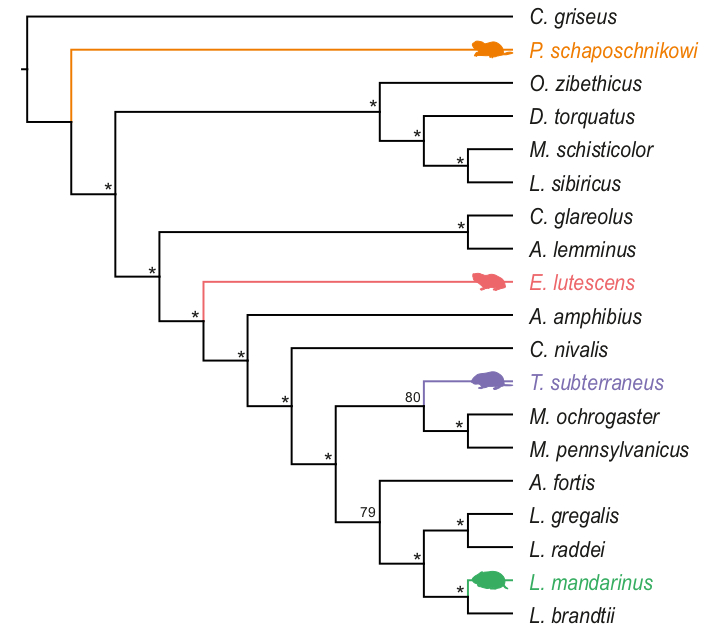
\includegraphics[width=0.5\textwidth]{RNA_tree_colour}
	\end{center}
	\caption{Филогенетическое дерево, построенное при использовании 112 ядерных белок-кодирующих генов}\label{tree_RNA}
\end{figure}

\subsection{Оценка уровня отбора} 


Мы провели поиск следов отбора в найденных нами ортологичных генах независимо для каждой линии подземных грызунов (рис. \ref{RNA_trees_sep}). Однако, генов с достоверными отличиями обнаружено не было. 

\begin{figure}[h!]
	\begin{center}
		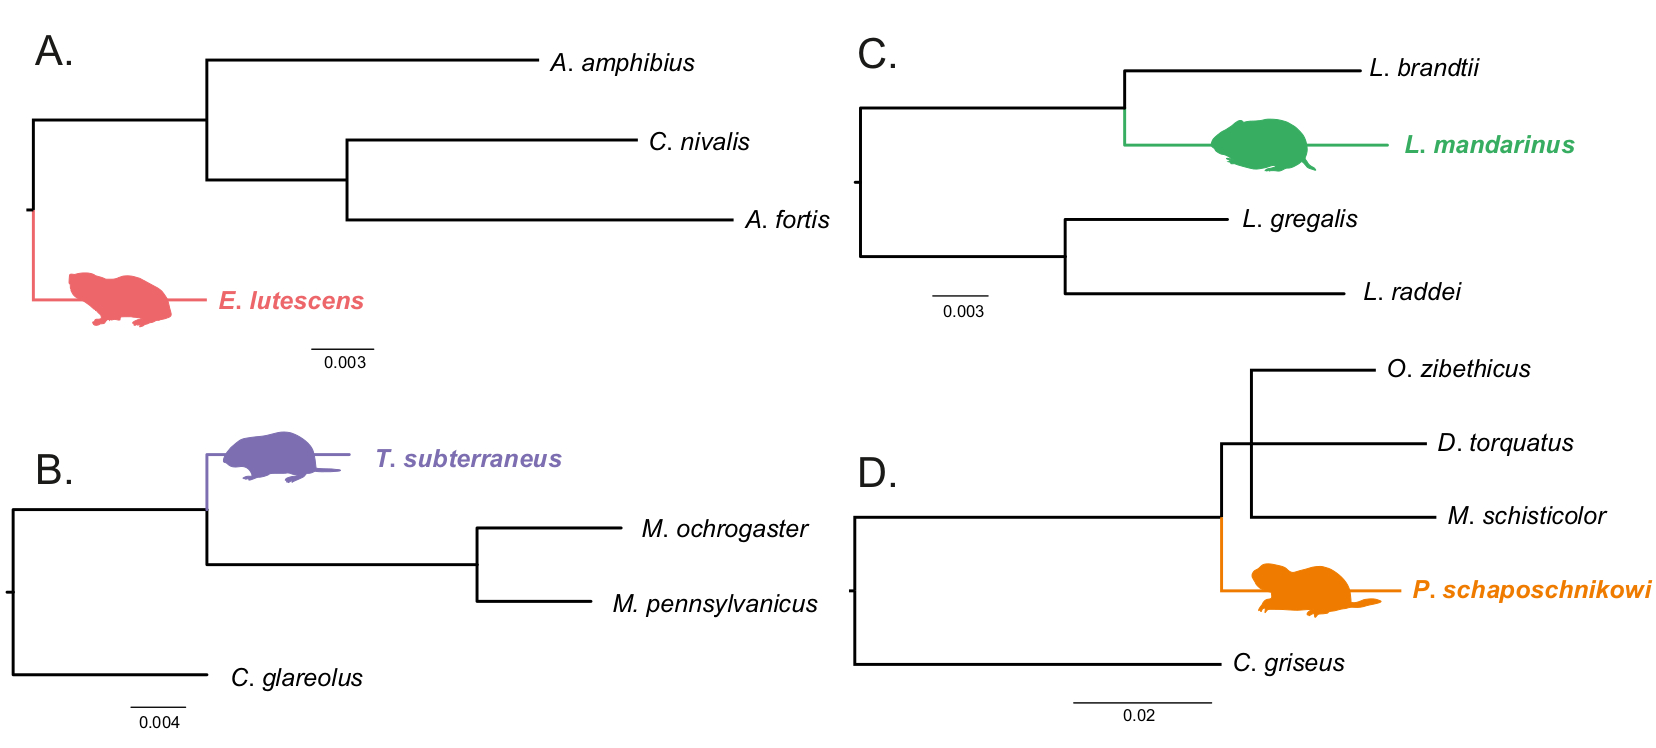
\includegraphics[width=\textwidth]{separate trees_RNA_color}
	\end{center}
	\caption{Подземные виды (выделены цветом) и филогенетически близкие наземные виды для поиска следов отбора. }\label{RNA_trees_sep}
\end{figure}


\subsection{Анализ частоты несинонимичных замен}

Сравнение частот несинонимичных замен между подземными и наземными видами не показало достоверных различий (рис. \ref{sub_RNA}). Также нами не было обнаружено отдельных генов  или позиций, в которых частоты будут достоверно различаться. 

\begin{figure}[h!]
	\begin{center}
		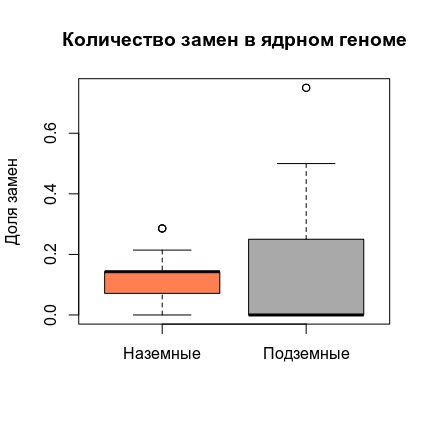
\includegraphics[width=0.5\textwidth]{sub_rna}
	\end{center}
	\caption{Оценка частот несинонимичных замен у подземных и наземных грызунов.}\label{sub_RNA}
\end{figure}

\subsection{Оценка параллельных аминокислотных замен}

При изучении полученных нами ядерных генов мы повторили подход поиска параллельных аминокислотных замен. Нами были обнаружены замены в нескольких генах, где у подземных грызунов она замещалась другой идентичной для всех (таблица \ref{rna_substitution_all}) и заменялись в той же позиции, но различными аминокислотами (таблица \ref{rna_substitution_diff}). Среди них оказались достоверные замены в генах \textit{Rad23b} и \textit{Pycr2}. 

\begin{table}[]
	\caption{Параллельные замены у подземных грызунов, обнаруженные в ядерных генах}\label{rna_substitution_all} \vspace{5mm}
	
	\begin{center}
	\begin{tabular}{|l|c|c|c|c|c|c|c|c|c|c}
		\hline
		\multicolumn{1}{|r|}{Ген} & \textit{Rad23b} & \textit{Hikeshi} & \textit{Mrps14} & \textit{Pycr2} & \textit{GTPBP2} & \textit{Snapc2} \\ \hline
		Вид   / позиция & 121 & 189 & 5 & 314 & 30 & 204  \\ \hline
		Наземные виды &  Thr & Ala & Val & Ala & Val & Glu  \\ \hline
		\textit{E. lutestence}  & -- & Thr & -- & Thr  & Met & Gly  \\ \hline
		\textit{P. schaposchnikowi}  & Ala & -- & Met & Thr & Met & Gly  \\ \hline
		\textit{L. mandarinus}  & -- & -- & -- & --  & -- & --  \\ \hline
		\textit{T. subterraneus} & Ala & Thr  & Met & -- & -- & -- \\ \hline
	\end{tabular}
\end{center}
\end{table}


\begin{table}[]
	\caption{Дивергентные замены у подземных грызунов, обнаруженные в ядерных генах}\label{rna_substitution_diff} \vspace{5mm}
	
	\begin{center}
	\begin{tabular}{|l|c|c|c|c|c|c|c|c|c|c}
		\hline
		\multicolumn{1}{|r|}{Ген} & \textit{Erp29} & \textit{Zadh2} & \textit{Ccdc86} & \textit{Ttll12} \\ \hline
		Вид   / позиция & 255 & 162 & 125 &  91 \\ \hline
		Наземные виды & Ala & Ala & His & Gln \\ \hline
		\textit{E. lutestence} & Val & Val & -- & -- \\ \hline
		\textit{P. schaposchnikowi} & Thr & Thr & Pro & Arg \\ \hline
		\textit{L. mandarinus} & -- & -- & Arg  & -- \\ \hline
		\textit{T. subterraneus} & -- & -- & -- & Lys \\ \hline
	\end{tabular}
\end{center}
\end{table}
